\documentclass[11pt]{article}
\usepackage[T1]{fontenc}
\usepackage[utf8]{inputenc}
\usepackage{lmodern}
\usepackage[a4paper,margin=29mm]{geometry}
\usepackage{amsmath,amssymb,amsthm,mathtools}
\usepackage{enumitem,booktabs,microtype}
\usepackage{needspace}
\usepackage{xcolor}
\usepackage{tikz}
\usetikzlibrary{arrows.meta}
\usepackage[unicode,pdfencoding=auto,psdextra]{hyperref}
\usepackage[nameinlink,capitalise,noabbrev]{cleveref}
\hypersetup{colorlinks=true,linkcolor=blue!45!black,citecolor=green!35!black,
  urlcolor=blue!55!black,
  pdftitle={Bounded recovery for modular spectral averages},
  pdfauthor={OpenAI},pdfsubject={Triviality of bicentralizers for type III1 factors}}
\urlstyle{same}
\pdfgentounicode=1
\pdfinfoomitdate=1
\pdftrailerid{}
\pdfsuppressptexinfo=15
\newtheorem{theorem}{Theorem}[section]
\numberwithin{equation}{section}
\newtheorem{proposition}[theorem]{Proposition}
\newtheorem{lemma}[theorem]{Lemma}
\newtheorem{corollary}[theorem]{Corollary}
\theoremstyle{definition}
\newtheorem{definition}[theorem]{Definition}
\theoremstyle{remark}
\newtheorem{remark}[theorem]{Remark}
\newcommand{\C}{\mathbb C}
\newcommand{\R}{\mathbb R}
\newcommand{\N}{\mathbb N}
\newcommand{\Z}{\mathbb Z}
\newcommand{\B}{\mathcal B}
\DeclareMathOperator{\BC}{BC}
\DeclareMathOperator{\id}{id}
\DeclareMathOperator{\supp}{supp}
\DeclareMathOperator{\Aut}{Aut}
\DeclareMathOperator{\Dom}{Dom}
\DeclareMathOperator{\linspan}{span}
\DeclarePairedDelimiter{\norm}{\lVert}{\rVert}
\DeclarePairedDelimiter{\abs}{\lvert}{\rvert}
\DeclarePairedDelimiter{\set}{\{}{\}}
\setlist[enumerate]{label=\textup{(\roman*)},leftmargin=2em}
\setlength{\emergencystretch}{1.5em}
\allowdisplaybreaks[1]

\title{Bounded recovery for modular spectral averages}
\author{OpenAI}
\date{September 23, 2026}
\begin{document}
\maketitle
\begin{abstract}
We prove a bounded spectral recovery theorem for a von Neumann algebra with
a faithful normal state whose centralizer consists only of scalars. A positive
averaged squared norm for an arbitrary bounded Hilbert-space operator on
shrinking modular spectral bands can be recovered on uniformly bounded algebra
elements with shrinking spectral support. We apply this theorem to spectral
intertwining rigidity and obtain an alternative proof of bicentralizer triviality
for type $\mathrm{III}_1$ factors with separable predual.
\end{abstract}
\section{Introduction}

Spectral localization in the standard Hilbert space of a von Neumann
algebra does not by itself produce uniformly bounded elements of the
algebra. This distinction matters when an argument starts with spectral
vectors but its asymptotic identities apply only to bounded operator
sequences. Our main analytical result, \Cref{rec:bounded}, provides a
bounded recovery principle for this situation.

Let $M$ be a von Neumann algebra with a faithful normal state $\phi$.
Write $M_\phi$ for the fixed-point algebra of its modular automorphism
group $\sigma^\phi$. We call $\phi$ ergodic when $M_\phi=\C1$.
On the standard Hilbert space $H=L^2(M)$, put
$\xi=\phi^{1/2}$, $D=\log\Delta_\phi$, and $U_t=e^{itD}$.
For an arbitrary fixed $T\in\B(H)$, consider unit vectors supported in
spectral intervals of $D$ shrinking to a real number $s$.
\Cref{rec:bounded} shows that a positive limiting averaged value of
$\norm{TU_th}^2$ on these vectors can be recovered as a positive value of
$\norm{Tv\xi}^2$ on a sequence of uniformly bounded $v\in M$.
The recovered vectors remain in intervals shrinking to $s$, with widths
at most four times the original widths. The averaging uses a fixed
translation-invariant mean obtained from symmetric interval averages.
The exact quantifiers and mean are given in
\Cref{mod:average,rec:bounded}.

The only structural assumption in this recovery theorem is
$M_\phi=\C1$; neither a bicentralizer condition nor a second action is
required. This assumption supplies a broad class of applications:
Marrakchi and Vaes proved that ergodic faithful normal states form a
dense $G_\delta$ in the normal state space of every type
$\mathrm{III}_1$ factor with separable predual
\cite[Theorem~A]{MarrakchiVaes2024}.

\paragraph{Bicentralizers and prior work.}
We use the predual convention
\[
  (w\phi)(y)=\phi(yw),\qquad
  (\phi w)(y)=\phi(wy).
\]
The bicentralizer $\BC(M,\phi)$ consists of those $a\in M$ for which
$[a,w_n]\to0$ strongly whenever $(w_n)$ is uniformly bounded and
$\norm{w_n\phi-\phi w_n}_{M_*}\to0$.
Connes' bicentralizer conjecture asserts that this algebra is scalar
for every type $\mathrm{III}_1$ factor with separable predual.
Connes developed the problem in his classification program for injective
factors \cite{Connes1980,Connes1985}. Haagerup proved the amenable case,
completing the uniqueness theorem for the injective type
$\mathrm{III}_1$ factor \cite{Haagerup1987}.

Haagerup also related triviality to the existence of a faithful normal
state with irreducible centralizer, meaning
$(M_\phi)'\cap M=\C1$ \cite[Theorem~3.1]{Haagerup1987}.
Together with Popa's work on maximal abelian subalgebras
\cite{Popa1981}, this connects the problem to expected subalgebras;
the expected-masa equivalence is stated in
\cite[Corollary~3.6]{HI2017}.
Important nonamenable cases include Houdayer's theorem for free Araki--Woods factors
\cite{Houdayer2009} and the semisolid factors treated by Houdayer and
Isono \cite[Theorem~3.7]{HI2017}.
An irreducible centralizer in these results is different from the scalar
centralizer assumed in our recovery theorem.

Houdayer and Isono proved that a nonscalar bicentralizer of a separable
type $\mathrm{III}_1$ factor is itself a type $\mathrm{III}_1$ factor
and equals its own bicentralizer for the restricted state
\cite[Proposition~3.4 and Theorem~3.5]{HI2017}.
Ando, Haagerup, Houdayer, and Marrakchi established the canonical relative
bicentralizer flow \cite[Theorem~A]{AHHM2020}, following the flow
construction of Haagerup and its independent discovery by Marrakchi.
Marrakchi proved that every nonidentity time of the absolute flow is
ergodic, without a fullness assumption
\cite[Theorem~D]{Marrakchi2020}. His subsequent work develops the
binormal-state and relative-core machinery
\cite{Marrakchi2025,Marrakchi2026}.

\paragraph{The absolute application and the recent announcement.}
Houdayer and Marrakchi have announced triviality of the bicentralizer
for every type $\mathrm{III}_1$ factor admitting a faithful normal
state, with no separability condition in the theorem statement
\cite[Theorem~G]{HoudayerMarrakchi2026}.
The application proved here is an alternative proof of the
separable-predual instance of that conclusion.

\begin{theorem}\label{thm:main}
Let $M$ be a type $\mathrm{III}_1$ factor with separable predual and let
$\phi$ be any faithful normal state on $M$. Then
\[
  \BC(M,\phi)=\C1.
\]
\end{theorem}

By \cite[Corollary~3.6]{HI2017}, \Cref{thm:main} also implies that every
type $\mathrm{III}_1$ factor with separable predual admits a maximal
abelian subalgebra with a faithful normal conditional expectation.
This is an existence statement for the factor; the expectation need not
preserve the scalar-centralizer state used in bounded recovery.

The independent analytical contribution is the bounded recovery theorem, which applies
to arbitrary $T$ without assuming a bicentralizer intertwining law.
Houdayer and Marrakchi obtain the same symmetric spectral relation used
below through multiplication isometries and a singular KMS state on the
continuous core
\cite[Section~8.4, Propositions~8.8--8.10]{HoudayerMarrakchi2026}.
Here modular averaging and bounded recovery lead to that relation through
two interval estimates.

Houdayer and Marrakchi explicitly disclose assistance from
\emph{GPT-5.6 Sol} and \emph{GPT-6 Astra}
\cite[p.~7]{HoudayerMarrakchi2026}. They credit Sol with counterexample
exploration and an initial strict-outerness argument, and Astra with
the singular tracial-state ingredient in their resonance strategy.
They describe checking and rewriting the proofs and retaining
responsibility for them. These are their stated contributions to that
work, whose relative tracial-action theory is also developed in the paper.

\paragraph{The rigidity statement.}
A continuous action on $M$ means a $u$-continuous action on its
automorphism group. Bounded recovery gives the following spectral proof
of rigidity.

\begin{theorem}[Spectral intertwining rigidity]\label{thm:rigidity}
Let $M$ be a von Neumann algebra with a faithful normal state $\phi$ such
that $M_\phi=\C1$. Let $b:\R\curvearrowright M$ be a continuous
$\phi$-preserving action. Suppose that, for every $s\in\R$, every uniformly
bounded sequence $(w_n)$ in $M$, and every $a\in M$,
\begin{equation}\label{eq:flow-property}
  \norm{\phi w_n-e^s w_n\phi}_{M_*}\longrightarrow0
  \quad\Longrightarrow\quad
  w_na-b_s(a)w_n\longrightarrow0
  \quad\text{strongly}.
\end{equation}
Then $b_s=\id_M$ for every $s\in\R$.
\end{theorem}

The conclusion also follows from the announced absolute theorem.
Indeed, at $s=0$, hypothesis \eqref{eq:flow-property} implies
$\BC(M,\phi)=M$. If $M\ne\C1$, its scalar centralizer makes it a
type $\mathrm{III}_1$ factor by
\cite[Lemma~2.1]{MarrakchiVaes2024}; the announced theorem would then
force $M=\C1$. Our proof instead derives \Cref{thm:rigidity} directly
from bounded recovery and uses it to prove \Cref{thm:main}.
For that application to a self-bicentralizing factor, the modular
centralizer is scalar, the bicentralizer flow satisfies
\eqref{eq:flow-property}, and that flow is ergodic. A trivial ergodic
action has scalar underlying algebra.

\paragraph{Recovery and the spectral argument.}
The recovery proof combines modular averaging with the fourth-moment
and polar-cutoff devices of Haagerup and Musat
\cite[Equation~(2.10), Lemma~2.6, and Remark~2.8]{HaagerupMusat2007}.
The strategy of recovering bounded witnesses by randomization,
fourth-moment control, and truncation appears in the tracial spectral-gap
argument of Ioana and Vaes \cite[pp.~127--130]{IoanaVaes2015}.
Related fourth-moment control underlies Marrakchi's binormal-state
implementation \cite[Section~2, Claim~2.2]{Marrakchi2025}.
Here modular orbit averages supply the moment bounds, and a final Fourier
filter restores the shrinking spectral bands.
The averaging time is chosen separately for each initial bounded
representative of a spectral vector; these representatives need not be
uniformly bounded.
Norm convergence in the predual controls a varying second-moment
operator, and independent circle phases give a uniform fourth-moment
bound. One fixed polar truncation threshold then suffices. Fourier
localization restores the spectral support without increasing operator
norms by a factor depending on the width of the spectral interval.
The Fourier operations belong to the standard spectral-subspace
framework for automorphism groups \cite{Arveson1974}; the bounds needed
here are proved explicitly.

For the spectral application, implement the state-preserving action by
$V_s(a\xi)=b_s(a)\xi$ and write $V_s=e^{isQ}$. These unitaries commute
with $U_t$, so $(D,Q)$ has a joint spectral support $\mathcal S\subset\R^2$.
The recovered bounded sequences let \eqref{eq:flow-property} force
averaged intertwining defects to vanish on bands shrinking to a fixed
modular energy. A spectral partition then gives an interval estimate
without requiring a rate uniform in that energy. Applying this estimate
twice, with the operators interchanged and the time reversed, gives
\[
  \exp\bigl(i(r\ell+qp)\bigr)=1
  \qquad ((r,p),(q,\ell)\in\mathcal S).
\]
This symmetric relation is the final rigidity mechanism. It forces the
joint support to be countable or to lie on a coordinate axis.
Scalarity of the modular centralizer excludes nonzero modular
eigenvalues, by the bounded-eigenoperator extraction and KMS argument of
\cite[Lemma~2.1]{MarrakchiVaes2024}, leaving only the axis on which the
flow generator vanishes.

\paragraph{Organization.}
\Cref{sec:bicentralizers} records the established bicentralizer inputs
and reduces \Cref{thm:main} to \Cref{thm:rigidity}.
\Cref{sec:modular} proves the modular and averaging preliminaries.
\Cref{sec:recovery} proves \Cref{rec:bounded}, and
\Cref{sec:rigidity} completes the spectral argument.

\section{Bicentralizers and the reduction}\label{sec:bicentralizers}

We recall the definition to fix both the topology and the quantifiers.
For a faithful normal state $\phi$, put
$\norm{x}_\phi=\phi(x^*x)^{1/2}$.
The bicentralizer consists of those $a\in M$ for which, for every
$\varepsilon>0$, there is $\delta>0$ such that
\[
  u\in\mathcal U(M),\quad
  \norm{u\phi-\phi u}_{M_*}<\delta
  \quad\Longrightarrow\quad
  \norm{u^*au-a}_\phi<\varepsilon.
\]
This is Haagerup's unitary formulation of the usual bicentralizer
\cite[proof of Lemma~1.2]{Haagerup1987}.
Equivalently, its elements asymptotically commute strongly with every
uniformly bounded sequence that asymptotically centralizes $\phi$ in
predual norm. We use established structural results in this equivalent
form.

\begin{proposition}[Established bicentralizer results]\label{bc:inputs}
Let $M$ be a type $\mathrm{III}_1$ factor with separable predual and
$\phi$ a faithful normal state.
\begin{enumerate}
\item\label{bc:reduction}
If $B=\BC(M,\phi)$ is nonscalar, then $B$ is a type
$\mathrm{III}_1$ subfactor with a normal $\phi$-preserving conditional
expectation, and
\[
  \BC(B,\phi|_B)=B.
\]
\item\label{bc:flow}
There is a continuous $\phi$-preserving action
$\beta^\phi:\R_+^*\curvearrowright\BC(M,\phi)$ characterized by
\[
  \norm{w_n\phi-\lambda\phi w_n}_{M_*}\longrightarrow0
  \quad\Longrightarrow\quad
  w_na-\beta^\phi_\lambda(a)w_n\longrightarrow0
  \quad *\text{-strongly}
\]
for every $\lambda>0$, every uniformly bounded sequence $(w_n)$ in $M$,
and every $a\in\BC(M,\phi)$.
\item\label{bc:ergodicity}
The fixed-point algebra of $\beta^\phi$ is $\C1$.
\end{enumerate}
\end{proposition}

\begin{proof}[Sources and hypotheses]
The restricted-state identity in \ref{bc:reduction} is
\cite[Proposition~3.4]{HI2017}; the type dichotomy and expectation are
\cite[Theorem~3.5]{HI2017}. The bicentralizer is globally invariant under
the modular group by \cite[Proposition~3.3]{HI2017}, so its canonical
expectation preserves $\phi$.
These results impose no amenability or fullness hypothesis.

For \ref{bc:flow}, apply \cite[Theorem~A(ii)]{AHHM2020} to the identity
inclusion $M\subset M$. Continuity is part of the flow construction.
The expectation-preservation identity in
\cite[Theorem~A(iv)]{AHHM2020} specializes to preservation of $\phi$,
because the relative commutant is $\C1$.

Finally, \cite[Theorem~D]{Marrakchi2020} states, for any $\sigma$-finite type
$\mathrm{III}_1$ factor, that every $\beta^\phi_\lambda$ with
$\lambda\ne1$ is ergodic. This is stronger than \ref{bc:ergodicity}.
Fullness is not assumed in this Theorem.
\end{proof}

\begin{proof}[Proof of \Cref{thm:main}, assuming \Cref{thm:rigidity}]
Suppose that $\BC(M,\phi)$ is nonscalar. Replace $(M,\phi)$ by
$(B,\phi|_B)$ using \Cref{bc:inputs}\ref{bc:reduction}.
The restricted state is faithful and normal.
The predual is still separable: if $E:M\to B$ is the normal expectation,
$B_*\ni\rho\mapsto\rho\circ E\in M_*$ is an isometric embedding.
We may therefore assume
\[
  \BC(M,\phi)=M,\qquad M\ne\C1.
\]

Every unitary $u\in M_\phi$ centralizes $\phi$ exactly. The unitary
definition of the bicentralizer gives $u^*au=a$ for every $a\in M$.
Since unitaries span $M_\phi$, and $M$ is a factor, it follows that
$M_\phi=\C1$.

Set $b_s=\beta^\phi_{e^{-s}}$.
The premise of \eqref{eq:flow-property} is equivalent to
\[
  \norm{w_n\phi-e^{-s}\phi w_n}_{M_*}\longrightarrow0.
\]
\Cref{bc:inputs}\ref{bc:flow} therefore gives exactly
\eqref{eq:flow-property}, and also continuity and state preservation.
By \Cref{thm:rigidity}, $b$ is trivial. By
\Cref{bc:inputs}\ref{bc:ergodicity}, it is ergodic. Hence $M=\C1$,
contradicting the reduction.
The contradiction applies to every original pair $(M,\phi)$.
\end{proof}

\section{Modular localization and averaging}\label{sec:modular}

The recovery argument requires two kinds of control: modular spectral
localization must imply a predual norm estimate, and modular averaging
must control the moments of an operator even when its norm is large.
We establish these facts here. The two norm limits in
\Cref{mod:means} will control different terms in the fourth-moment
expansion in \Cref{sec:recovery}.

Throughout this Section $M$ is a von Neumann algebra with a faithful
normal state $\phi$. Let $H=L^2(M)$ be its standard Hilbert space,
$\xi=\phi^{1/2}$ its cyclic separating unit vector, and
\[
  L(a)h=ah,\qquad R(a)h=ha,\qquad
  D=\log\Delta_\phi,\qquad U_t=e^{itD}.
\]
Write $E_D$ for the spectral resolution of $D$ and $J$ for the modular
conjugation. Inner products are linear in the first variable.
We use the standard modular theory of \cite{Takesaki2003}.
We write $\sigma_t=\sigma^\phi_t$.
Standard modular theory gives
\begin{equation}\label{eq:modular-identities}
  U_t(a\xi)=\sigma_t(a)\xi,\qquad
  e^{D/2}a\xi=\xi a,\qquad
  R(a)=JL(a)^*J.
\end{equation}
Indeed, $M\xi$ is contained in the domain of the closed Tomita operator
$S=J\Delta_\phi^{1/2}$, with $S(a\xi)=a^*\xi$.
Thus $\Delta_\phi^{1/2}a\xi=Ja^*\xi=\xi a$.
These standard-form conventions are also those of
\cite[Section~2.1]{AHHM2020}.

\begin{lemma}[From modular localization to predual norm]\label{mod:predual}
For $w\in M$ and $s\in\R$,
\begin{equation}\label{eq:predual-bound}
  \norm{\phi w-e^sw\phi}_{M_*}
  \le (1+e^{s/2})\norm{(e^{D/2}-e^{s/2})w\xi}.
\end{equation}
Consequently, if $(w_n)$ is uniformly bounded and the $D$-spectral
support of $w_n\xi$ is contained in
$[s-d_n,s+d_n]$ with $d_n\to0$, then the left side of
\eqref{eq:predual-bound} tends to zero.
\end{lemma}

\begin{proof}
Put $c=e^{s/2}$ and $\eta=\xi w-cw\xi$.
By \eqref{eq:modular-identities},
$\eta=(e^{D/2}-c)w\xi$, and
$J\eta=w^*\xi-c\xi w^*$.
For $\norm{y}\le1$, commutation of the left and right actions gives
\[
  \langle y\xi,\xi w^*\rangle
  =\langle y(\xi w),\xi\rangle.
\]
Starting from $\phi(wy)=\langle y\xi,w^*\xi\rangle$, replace
$w^*\xi$ by $c\xi w^*$, and then $\xi w$ by $cw\xi$.
The total error is at most $(1+c)\norm{\eta}$, while the resulting
expression is $c^2\phi(yw)$. Taking the supremum over $y$ proves the
estimate. The last assertion follows from
\[
  \norm{(e^{D/2}-e^{s/2})w_n\xi}
  \le \sup_{\abs{u-s}\le d_n}\abs{e^{u/2}-e^{s/2}}\,
       \norm{w_n\xi}.
  \qedhere
\]
\end{proof}

\begin{lemma}[Smooth spectral localization]\label{mod:localization}
Let $f\in C_c^\infty(\R)$, with Fourier convention
$f(u)=\int_{\R}g(t)e^{itu}\,dt$.
For $y\in M$, the weak integral
\[
  y_f=\int_{\R}g(t)\sigma_t(y)\,dt
\]
belongs to $M$ and satisfies
$\norm{y_f}\le\norm{g}_1\norm{y}$ and
$y_f\xi=f(D)y\xi$.
If $a\in M$ and $a\xi$ has compact $D$-spectral support, there is $a^\flat\in M$
such that
\begin{equation}\label{eq:right-multiplier}
  a\xi=\xi a^\flat.
\end{equation}
The same Fourier construction applies to any continuous
state-preserving action and its unitary implementation.
\end{lemma}

\begin{proof}
The inverse Fourier transform $g$ is integrable.
The bounded weak integral is defined by integration against normal
functionals, and its operator norm has the stated bound.
Applying it to $\xi$ and using the spectral theorem gives
$y_f\xi=f(D)y\xi$. This uses no operator norm continuity of the orbit.

If $K$ is a compact support for $a\xi$, choose $f\in C_c^\infty(\R)$
equal to $e^{-u/2}$ on a neighborhood of $K$, and put $a^\flat=a_f$.
Then \eqref{eq:modular-identities} and functional calculus give
\[
  \xi a^\flat=e^{D/2}a^\flat\xi
  =e^{D/2}f(D)a\xi=a\xi.
\]
All vectors in this computation belong to the domain of $e^{D/2}$;
in particular the filtered vector has compact spectral support.
The Fourier argument for another state-preserving action is identical.
\end{proof}

For the rest of this Section assume $M_\phi=\C1$.
Let $\mu_k$ be uniform probability measure on $[-k,k]$, for
$k\in\N$.

\begin{lemma}[Two norm ergodic limits]\label{mod:means}
For every $y\in M$ and $\psi\in M_*$,
\begin{align}
  \int\sigma_t(y)\xi\,d\mu_k(t)&\longrightarrow\phi(y)\xi
       &&\text{in }H,\label{eq:hilbert-mean}\\
  \int\psi\circ\sigma_{-t}\,d\mu_k(t)&\longrightarrow\psi(1)\phi
       &&\text{in }M_*.\label{eq:predual-mean}
\end{align}
\end{lemma}

\begin{proof}
The unitary mean ergodic theorem gives a norm limit for the vectors in
\eqref{eq:hilbert-mean}. The corresponding operator averages have norm
at most $\norm{y}$. For each fixed $u$, translating the interval changes
their averages in operator norm by at most
$\abs{u}\norm{y}/k$ for all sufficiently large $k$.
Every weak operator cluster point is consequently fixed by $\sigma$,
hence scalar. Evaluation under $\phi$ identifies it as $\phi(y)1$.
This identifies the Hilbert norm limit and proves
\eqref{eq:hilbert-mean}.

The action on $M_*$ is norm continuous on each functional.
For positive normal functionals this follows from their realization as
vector functionals in standard form and the strong continuity of $U$;
linear decomposition gives the general case.
The predual averages are therefore Bochner integrals and are
contractions. Let
\[
  \mathcal N=\overline{\linspan}^{\,\norm{\cdot}}
   \{\rho\circ\sigma_u-\rho:\rho\in M_*,\ u\in\R\}.
\]
Its annihilator in $(M_*)^*=M$ is $M_\phi=\C1$.
The Hahn--Banach theorem implies
$\mathcal N=\{\psi\in M_*:\psi(1)=0\}$.
The averages tend to zero in norm on each generator of $\mathcal N$,
by the interval boundary estimate, and hence on all of $\mathcal N$ by
contractivity. They fix $\phi$. Apply this to $\psi-\psi(1)\phi$ to
obtain \eqref{eq:predual-mean}.
\end{proof}

Fix a free ultrafilter $\omega$ on $\N$. For a bounded continuous scalar
function $f$ define
\[
  m_t f(t)=\lim_{k\to\omega}\int f(t)\,d\mu_k(t).
\]
This positive normalized mean is invariant under translations and under
$t\mapsto-t$. For a bounded continuous $H$-valued function $F$, put
\[
  \norm{F}_{\mathrm{av}}
  =\bigl(m_t\norm{F(t)}^2\bigr)^{1/2}.
\]
The triangle inequality follows from the corresponding inequalities for
the finite interval integrals. Thus this is a seminorm.

\Needspace{6\baselineskip}
\begin{lemma}[Operator averaging]\label{mod:average}
For $S\in\B(H)$, define $P(S)$ by
\[
  \langle P(S)h,k\rangle
  =m_t\langle U_t^*SU_th,k\rangle.
\]
Then $P$ is a positive unital contraction, $P(S)$ commutes with every
spectral projection of $D$, and
\begin{equation}\label{eq:scalar-average}
  P(L(a))=\phi(a)1\qquad(a\in M).
\end{equation}
In particular,
\begin{equation}\label{eq:quadratic-average}
  \norm{t\mapsto SU_th}_{\mathrm{av}}^2
  =\langle P(S^*S)h,h\rangle.
\end{equation}
\end{lemma}

\begin{proof}
The bounded sesquilinear form defines $P(S)$, with
$\norm{P(S)}\le\norm{S}$. Positivity and unitality follow directly from
the mean. Translation invariance gives $U_u^*P(S)U_u=P(S)$ for every
$u$, hence commutation with the spectral projections of $D$.
For $S=L(a)$ the averages and their weak limits belong to the weakly
closed algebra $L(M)$, since
$U_t^*L(a)U_t=L(\sigma_{-t}(a))$.
The fixed-point algebra is scalar, and evaluation at $\xi$ gives
\eqref{eq:scalar-average}. Equation \eqref{eq:quadratic-average} is the
definition applied to $S^*S$.
No normality of $P$ is asserted or needed.
\end{proof}

\section{Recovering bounded operators from spectral vectors}
\label{sec:recovery}

\Cref{rec:bounded} converts a positive averaged quantity on narrow modular
spectral bands into a positive quantity on uniformly bounded operators.
Its proof uses both norm limits in \Cref{mod:means}: the Hilbert-space
limit controls one fourth-moment term, and the predual limit controls the
other.  No uniform operator norm bound is required for the initial
representatives of the spectral vectors.
Randomization, fourth-moment control, truncation, and selection of a
bounded witness occur together in the tracial spectral-gap argument of
Ioana and Vaes \cite[proof of the appendix theorem, pp.~129--130]{IoanaVaes2015}.
Related fourth-moment control gives equi-integrability in Marrakchi's
binormal-state implementation \cite[Section~2, Claim~2.2]{Marrakchi2025}.
We use the fourth-moment and polar-cutoff devices of Haagerup and Musat
\cite[Lemma~2.6 and Remark~2.8]{HaagerupMusat2007}, with moment bounds
supplied by modular orbit averages against the given state. The final
Fourier localization retains the shrinking spectral band.

\begin{theorem}[Bounded recovery]
\label{rec:bounded}
Let $M$ be a von Neumann algebra with a faithful normal state $\phi$ such
that $M_\phi=\C1$.  Use the standard-space notation and the fixed mean $m$
of \Cref{mod:average}.  Fix $T\in\B(H)$ and $s\in\R$.  Suppose that
$\delta_n>0$ tends to zero and that $h_n\in H$ are unit vectors with
$D$-spectral support in $[s-\delta_n,s+\delta_n]$.  If
\begin{equation}
\label{eq:recovery-positive}
 \limsup_{n\to\infty}m_t\norm{TU_th_n}^{2}>0,
\end{equation}
then there are a subsequence $(n_j)$, elements $v_j\in M$, and constants
$C_*<\infty$ and $\eta>0$ such that, for every $j$,
\[
 \norm{v_j}\le C_*,\qquad
 \norm{Tv_j\xi}\ge\eta,
\]
and $v_j\xi$ has $D$-spectral support in
$[s-4\delta_{n_j},s+4\delta_{n_j}]$.
\end{theorem}

\begin{proof}
We use the same family of Fourier filters to localize the initial bounded
approximations and to restore localization after polar truncation.
Choose $f_0\in C_c^\infty(\R)$ such that
\[
 0\le f_0\le1,\qquad f_0=1\text{ on }[-1,1],\qquad
 \supp f_0\subset[-2,2],
\]
and write $f_0(u)=\int_\R g_0(t)e^{itu}\,dt$, with $g_0$ a Schwartz
function.  For $\rho>0$, set
\[
 f_\rho(u)=f_0\bigl((u-s)/\rho\bigr),\qquad
 g_\rho(t)=\rho e^{-ist}g_0(\rho t).
\]
Then $f_\rho(u)=\int_\R g_\rho(t)e^{itu}\,dt$ and
\begin{equation}
\label{eq:recovery-kernel}
 \norm{g_\rho}_1=\norm{g_0}_1=:C_1
 \quad\text{for every }\rho>0.
\end{equation}
By \Cref{mod:localization}, the weak integral
\[
 \mathcal F_\rho(x)
   =\int_\R g_\rho(t)\sigma_t(x)\,dt\in M
\]
satisfies
\begin{equation}
\label{eq:recovery-filter}
 \mathcal F_\rho(x)\xi=f_\rho(D)x\xi,
 \qquad \norm{\mathcal F_\rho(x)}\le C_1\norm{x}.
\end{equation}
In particular, its vector has spectral support in
$[s-2\rho,s+2\rho]$.

\smallskip
\noindent\emph{Approximation by bounded representatives.}
By \Cref{eq:recovery-positive}, after passing to a subsequence and
reindexing, there is $\gamma>0$ such that
\[
 m_t\norm{TU_th_n}^{2}\ge4\gamma\qquad(n\ge1).
\]
Since $M\xi$ is dense in $H$, approximate $h_n$ by $x_n\xi$ and apply
$f_{\delta_n}(D)$.  This multiplier fixes $h_n$ and is a contraction.
Thus the vectors $\mathcal F_{\delta_n}(x_n)\xi$ approximate $h_n$ as
closely as desired.  Normalize them, obtaining $y_n\in M$ with
$\norm{y_n\xi}=1$ and spectral support in
$[s-d_n,s+d_n]$, where $d_n=2\delta_n$.  Choose the approximations so that
$\norm{y_n\xi-h_n}\to0$ and
\begin{equation}
\label{eq:recovery-defect}
 m_t\norm{TU_ty_n\xi}^{2}\ge2\gamma\qquad(n\ge1).
\end{equation}
This is possible because the averaged seminorm in
\Cref{mod:average} gives
\[
 \abs{\norm{t\mapsto TU_ty_n\xi}_{\mathrm{av}}
       -\norm{t\mapsto TU_th_n}_{\mathrm{av}}}
 \le\norm{T}\norm{y_n\xi-h_n}.
\]
Discard finitely many terms so that $d_n\le1$.  The modular identity
in \Cref{eq:modular-identities} gives
\begin{equation}
\label{eq:recovery-two-masses}
 \phi(y_n^*y_n)=1,\qquad
 \phi(y_ny_n^*)=\norm{e^{D/2}y_n\xi}^{2}\le e^{s+d_n}.
\end{equation}
There is no asserted uniform bound on $\norm{y_n}$.

\smallskip
\noindent\emph{Simultaneous defect and moment bounds.}
Fix $n$ for the moment, and write $y=y_n$.  With $\mu_k$ the uniform
probability measure on $[-k,k]$, define
\[
 \begin{aligned}
 A_k&=\int\sigma_t(y^*y)\,d\mu_k(t),&
 B_k&=\int\sigma_t(yy^*)\,d\mu_k(t),\\
 \psi(x)&=\phi(y^*xy),&
 \psi_k&=\int\psi\circ\sigma_{-t}\,d\mu_k(t).
 \end{aligned}
\]
We seek simultaneous control of $\phi(A_k^2)$ and $\psi_k(B_k)$, which
will bound the fourth moment after discretization. Here $\psi$ is a
normal state. State invariance gives the exact identity
\begin{equation}
\label{eq:recovery-functional}
 \psi_k(x)=
 \int\phi\bigl(\sigma_t(y)^*x\sigma_t(y)\bigr)\,d\mu_k(t).
\end{equation}
By the two ordinary norm limits in \Cref{mod:means},
\[
 A_k\xi\longrightarrow\xi,\qquad
 \norm{\psi_k-\phi}_{M_*}\longrightarrow0.
\]
Consequently $\phi(A_k^2)=\norm{A_k\xi}^{2}\to1$.  Although $B_k$
depends on $k$, it satisfies
\[
 \norm{B_k}\le\norm{y}^{2},\qquad
 \phi(B_k)=\phi(yy^*)\le e^{s+1},
\]
and hence
\begin{equation}
\label{eq:recovery-varying-test}
 \abs{\psi_k(B_k)-\phi(B_k)}
 \le\norm{\psi_k-\phi}_{M_*}\norm{y}^{2}\longrightarrow0.
\end{equation}
All these limits are taken with $n$ fixed.  For every sufficiently large
$k$ we may impose $\phi(A_k^2)\le2$ and
$\norm{\psi_k-\phi}_{M_*}\le\norm{y}^{-2}$ simultaneously.  It follows that
\begin{equation}
\label{eq:recovery-continuous-moments}
 \phi(A_k^2)+\psi_k(B_k)\le3+e^{s+1}.
\end{equation}
On the other hand, \Cref{eq:recovery-defect} and the definition of $m$
imply that the set of integers $k$ for which
\[
 \int\norm{T\sigma_t(y)\xi}^{2}\,d\mu_k(t)>\frac32\gamma
\]
belongs to the fixed free ultrafilter.  It therefore meets the cofinite
set on which \Cref{eq:recovery-continuous-moments} holds.  Choose one such
$k$, still for this fixed $n$.

We next replace this continuous average by a finite probability average.
Put $z_t=\sigma_t(y)$.  The three scalar functions
\[
 t\longmapsto\norm{Tz_t\xi}^{2},\qquad
 (t,u)\longmapsto\phi(z_t^*z_tz_u^*z_u),\qquad
 (t,u)\longmapsto\phi(z_t^*z_uz_u^*z_t)
\]
are continuous on the relevant compact interval or square.  Indeed,
$t\mapsto z_t$ is bounded and strong-star continuous, and products on
bounded sets preserve this continuity.  A common sufficiently fine
partition of $[-k,k]$, using its normalized interval lengths as weights,
therefore approximates all three integrals.  The product weights
approximate the double integrals defining $\phi(A_k^2)$ and
$\psi_k(B_k)$.  Thus there are finitely many times $t_i$ and weights
$p_i\ge0$, with $\sum_i p_i=1$, such that, writing
\[
 z_i=\sigma_{t_i}(y),\qquad
 A=\sum_i p_i z_i^*z_i,\qquad
 B=\sum_i p_i z_iz_i^*,
\]
we have
\begin{equation}
\label{eq:recovery-finite}
 \sum_i p_i\norm{Tz_i\xi}^{2}\ge\gamma,
 \qquad
 \phi(A^2)+\sum_i p_i\phi(z_i^*Bz_i)\le C,
 \qquad C:=4+e^{s+1}.
\end{equation}
The finite averages may depend on $n$; $\gamma$ and $C$ do not.  In
particular, no estimate on the rate in
\Cref{eq:recovery-varying-test} uniform in $n$ has been used.

\smallskip
\noindent\emph{Randomization and truncation.}
For this finite average, let $\epsilon_i$ be independent random variables
uniformly distributed on the complex unit circle, and set
\[
 z=\sum_i\sqrt{p_i}\,\epsilon_i z_i.
\]
The vector $z\xi$ is supported in $[s-d_n,s+d_n]$.  Independence and
vanishing first moments give
\[
 \mathbb E\norm{Tz\xi}^{2}
   =\sum_i p_i\norm{Tz_i\xi}^{2}\ge\gamma.
\]
The following expansion is the Steinhaus variant of the fourth-moment identity in
\cite[equation~(2.10) and Remark~2.8]{HaagerupMusat2007}, with
coefficients $\sqrt{p_i}z_i$. We include the expansion to keep track of
the order of the noncommuting factors. The two surviving pairings give
\begin{equation}
\label{eq:recovery-fourth}
 \mathbb E[(z^*z)^2]
  =A^2+\sum_i p_i z_i^*Bz_i
       -\sum_i p_i^2(z_i^*z_i)^2.
\end{equation}
The last sum subtracts the overlap of the pairings, where all four
indices agree.  Its summands are positive, so
\Cref{eq:recovery-finite} implies
\begin{equation}
\label{eq:recovery-fourth-bound}
 \mathbb E\phi((z^*z)^2)\le C.
\end{equation}

We next use the functional-calculus truncation underlying
\cite[Lemma~2.6, equations~(2.15)--(2.20)]{HaagerupMusat2007}.
For $K>0$, write $z=u\abs{z}$ in its polar decomposition and put
$z^{[K]}=u\min(\abs{z},K)$.  Then $\norm{z^{[K]}}\le K$ and
\begin{equation}
\label{eq:recovery-truncation}
 \begin{aligned}
 \mathbb E\norm{(z-z^{[K]})\xi}^{2}
 &=\mathbb E\phi\bigl((\abs{z}-K)_+^2\bigr)\\
 &\le K^{-2}\mathbb E\phi(\abs{z}^{4})
 \le CK^{-2}.
 \end{aligned}
\end{equation}
This controls the vector error on the side required for the bounded
operator $T$.  No estimate for the adjoint truncation error is needed.

\smallskip
\noindent\emph{Restoring the spectral band and selecting realizations.}
Define the random element $v=\mathcal F_{d_n}(z^{[K]})\in M$.
By \Cref{eq:recovery-filter}, every realization satisfies
\begin{equation}
\label{eq:recovery-bounded-output}
 \norm{v}\le C_1K,
 \qquad v\xi=f_{d_n}(D)z^{[K]}\xi,
\end{equation}
and $v\xi$ is supported in $[s-2d_n,s+2d_n]$.  Since $f_{d_n}(D)$ fixes
$z\xi$ and has norm at most one, \Cref{eq:recovery-truncation} gives
\[
 \mathbb E\norm{v\xi-z\xi}^{2}\le CK^{-2}.
\]
The triangle inequality in the Hilbert space of square-integrable random
$H$-vectors now yields
\begin{equation}
\label{eq:recovery-fixed-cutoff}
 \bigl(\mathbb E\norm{Tv\xi}^{2}\bigr)^{1/2}
 \ge\sqrt\gamma-\frac{\norm{T}\sqrt C}{K}.
\end{equation}
Fix once and for all
\[
 K\ge2\norm{T}\sqrt{C/\gamma}.
\]
The hypothesis implies $T\ne0$, so $K$ can be chosen positive.  This
choice is independent of $n$ and ensures that the left-hand side of
\Cref{eq:recovery-fixed-cutoff} is at least $\sqrt\gamma/2$.

To select a realization, note that $z$ depends norm-continuously on the
finite phase torus and $z^{[K]}=zq_K(z^*z)$, where
\[
 q_K(r)=\min\{1,K/\sqrt r\}\quad(r>0),\qquad q_K(0)=1.
\]
Since $q_K$ is continuous on $[0,\infty)$, continuous functional calculus
makes the cutoff norm-continuous. The filter $\mathcal F_{d_n}$ is bounded
and linear, so $\norm{Tv\xi}^2$ is continuous on the compact phase torus.
It therefore attains a maximum at least its expectation.
Choose such a realization $v_n$ for each $n$. Then
\[
 \norm{v_n}\le C_1K,
 \qquad \norm{Tv_n\xi}\ge\frac{\sqrt\gamma}{2},
\]
and its spectral support lies in
$[s-2d_n,s+2d_n]=[s-4\delta_n,s+4\delta_n]$.
Restoring the subsequence notation proves \Cref{rec:bounded} with
$C_*=C_1K$ and $\eta=\sqrt\gamma/2$.
\end{proof}

\Cref{fig:bounded-recovery} summarizes the construction. The averaging
time depends on the initial representative, whereas the moment bound,
cutoff threshold, and Fourier-kernel norm are independent of the width
of its spectral band.
\begin{figure}[tbp]
\centering
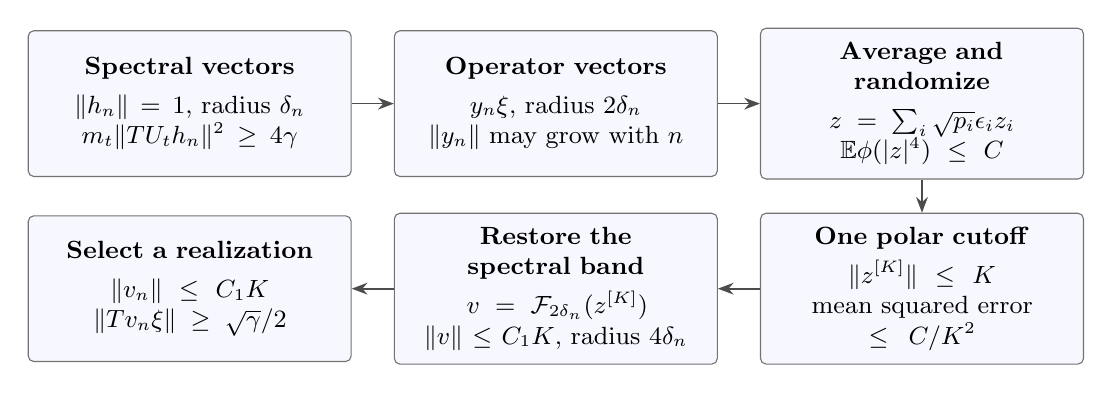
\begin{tikzpicture}[
  stage/.style={draw=black!55,rounded corners=2pt,fill=blue!3,
    text width=3.75cm,minimum height=1.85cm,align=center,
    inner sep=5pt,font=\small},
  flow/.style={-{Stealth[length=2mm]},semithick,draw=black!70}]
  \node[stage] (input) at (0,0) {
    \textbf{Spectral vectors}\\[3pt]
    $\norm{h_n}=1$, radius $\delta_n$\\
    $m_t\norm{TU_th_n}^2\ge4\gamma$};
  \node[stage] (approx) at (4.65,0) {
    \textbf{Operator vectors}\\[3pt]
    $y_n\xi$, radius $2\delta_n$\\
    $\norm{y_n}$ may grow with $n$};
  \node[stage] (random) at (9.3,0) {
    \textbf{Average and randomize}\\[3pt]
    $z=\sum_i\sqrt{p_i}\epsilon_i z_i$\\
    $\mathbb E\phi(|z|^4)\le C$};
  \node[stage] (cutoff) at (9.3,-2.35) {
    \textbf{One polar cutoff}\\[3pt]
    $\norm{z^{[K]}}\le K$\\
    mean squared error\\
    $\le C/K^2$};
  \node[stage] (filter) at (4.65,-2.35) {
    \textbf{Restore the spectral band}\\[3pt]
    $v=\mathcal F_{2\delta_n}(z^{[K]})$\\
    $\norm{v}\le C_1K$, radius $4\delta_n$};
  \node[stage] (output) at (0,-2.35) {
    \textbf{Select a realization}\\[3pt]
    $\norm{v_n}\le C_1K$\\
    $\norm{Tv_n\xi}\ge\sqrt\gamma/2$};
  \draw[flow] (input) -- (approx);
  \draw[flow] (approx) -- (random);
  \draw[flow] (random) -- (cutoff);
  \draw[flow] (cutoff) -- (filter);
  \draw[flow] (filter) -- (output);
\end{tikzpicture}
\caption{The construction in \Cref{rec:bounded}, after passing to the
subsequence with a positive averaged squared norm. Every band is centered at the
fixed modular energy $s$. The polar cutoff need not preserve that band;
the next Fourier filter restores it with radius $4\delta_n$. The constants
$C$, $K$, and $C_1$ are independent of $n$. The cutoff error is averaged
over the circle phases.}
\label{fig:bounded-recovery}
\end{figure}


\section{Spectral rigidity}
\label{sec:rigidity}

We now prove \Cref{thm:rigidity}. Throughout this Section, assume its
hypotheses and retain the modular notation and the symmetric mean from
\Cref{mod:average}. In particular, $M_\phi=\C1$. We use no ergodicity
assumption on $b$.

\subsection{From bounded recovery to an interval estimate}

When $a\xi=\xi a^\flat$, the identity $wa\xi=R(a^\flat)w\xi$ for
$w\in M$ writes the intertwining defect, at fixed $s$, as a bounded
operator applied to $w\xi$.

\begin{lemma}[Estimate at a spectral point]
\label{spec:point}
Let $a,a^\flat\in M$ satisfy $a\xi=\xi a^\flat$. For $s\in\R$, set
\[
 T_s=R(a^\flat)-L(b_s(a))\in\B(H).
\]
If $h_n\in H$ are unit vectors with $D$-spectral supports contained in
$[s-d_n,s+d_n]$, where $d_n>0$ and $d_n\to0$, then
\begin{equation}
 \norm{t\mapsto T_sU_th_n}_{\mathrm{av}}\longrightarrow0.
 \label{eq:point-estimate}
\end{equation}
\end{lemma}

\begin{proof}
If the conclusion fails, \Cref{rec:bounded}, applied to the fixed operator
$T_s$, gives a uniformly bounded sequence $v_n\in M$ such that the
$D$-spectral supports of $v_n\xi$ shrink to $s$ and
\[
 \norm{T_sv_n\xi}\geq\eta>0
 \qquad\text{for every }n.
\]
By \Cref{mod:predual},
\[
 \norm{\phi v_n-e^s v_n\phi}_{M_*}\longrightarrow0.
\]
The intertwining hypothesis \eqref{eq:flow-property} therefore gives
$(v_na-b_s(a)v_n)\xi\to0$. Since left and right multiplication commute,
\[
 T_sv_n\xi
   =v_n\xi a^\flat-b_s(a)v_n\xi
   =(v_na-b_s(a)v_n)\xi,
\]
a contradiction.
\end{proof}

The point estimate supplies no uniform rate in $s$. To pass to an interval,
we use the commutation of the averaged quadratic form with the spectral
projections of $D$.

\begin{lemma}[Estimate on an interval]
\label{spec:interval}
Let $a,a^\flat\in M$ satisfy $a\xi=\xi a^\flat$. For every nonempty compact
interval $I\subset\R$, every $c\in\C$, and every $h\in E_D(I)H$,
\begin{equation}
 \norm{t\mapsto (R(a^\flat)-cL(a))U_th}_{\mathrm{av}}
 \leq \norm{h}\sup_{s\in I}\norm{(b_s(a)-ca)\xi}.
 \label{eq:interval-estimate}
\end{equation}
\end{lemma}

\begin{proof}
Put
\[
 S=R(a^\flat)-cL(a),\qquad
 C=P(S^*S),\qquad
 B=\sup_{s\in I}\norm{(b_s(a)-ca)\xi}.
\]
The number $B$ is finite, and \Cref{mod:average} gives
\[
 \norm{t\mapsto SU_th}_{\mathrm{av}}^2=\langle Ch,h\rangle.
\]
Suppose that the asserted estimate fails. By homogeneity there is a unit
vector $h\in E_D(I)H$ with
\[
 \langle Ch,h\rangle=B^2+\varepsilon
 \qquad(\varepsilon>0).
\]
For each positive integer $n$, partition $I$ into finitely many disjoint
Borel intervals $J$ of diameter at most $1/n$. Since $C$ commutes with the
spectral projections of $D$,
\[
 \langle Ch,h\rangle
   =\sum_J\langle C E_D(J)h,E_D(J)h\rangle,
 \qquad
 \sum_J\norm{E_D(J)h}^2=1.
\]
Consequently, one nonzero spectral piece, after normalization, gives a unit
vector $h_n$ supported in $\overline{J_n}$ such that
\begin{equation}
 \langle Ch_n,h_n\rangle\geq B^2+\varepsilon.
 \label{eq:partition-gap}
\end{equation}
By compactness of $I$, after passing to a subsequence these supports lie in
intervals shrinking to a single point $s\in I$. This also covers a singleton
interval $I$.

Write $z=b_s(a)-ca$, so that $S=T_s+L(z)$. By \Cref{spec:point},
$\norm{t\mapsto T_sU_th_n}_{\mathrm{av}}\to0$. On the other hand,
\Cref{mod:average} gives the exact identity
\[
 \norm{t\mapsto L(z)U_th_n}_{\mathrm{av}}^2
 =\langle P(L(z^*z))h_n,h_n\rangle
 =\phi(z^*z)\leq B^2.
\]
The triangle inequality now yields
$\limsup_n\norm{t\mapsto SU_th_n}_{\mathrm{av}}\leq B$, contrary to
\eqref{eq:partition-gap}.
\end{proof}

\subsection{The joint spectral pairing}

State preservation gives a unitary implementation
\[
 V_s(a\xi)=b_s(a)\xi\qquad(a\in M).
\]
It is strongly continuous by the $u$-continuity of $b$: for $a\in M$,
\[
 \norm{V_s(a\xi)-a\xi}^2
 =2\phi(a^*a)-2\operatorname{Re}\phi(a^*b_s(a))\longrightarrow0
 \qquad(s\to0),
\]
and density extends this continuity to $H$. Since $b_s$ preserves $\phi$,
it commutes with the modular automorphism group. Thus $V_sU_t=U_tV_s$
for all $s,t$.
Write $V_s=e^{isQ}$. The self-adjoint operators $D$ and $Q$ strongly commute;
let $E$ be their joint spectral resolution and let $\mathcal S\subset\R^2$
be its closed support.

The joint spectral measure is concentrated on $\mathcal S$. Indeed, its
complement is a union of open sets with zero spectral projection, and the
countable base of $\R^2$ reduces this to a countable union. Hence
$E(\mathcal S)=1$, without any separability assumption on $H$.

\begin{lemma}[Joint spectral pairing]
\label{spec:pairing}
For every $(r,p),(q,\ell)\in\mathcal S$,
\begin{equation}
 \exp\bigl(i(r\ell+qp)\bigr)=1.
 \label{eq:spectral-pairing}
\end{equation}
\end{lemma}

\begin{proof}
Fix $\delta>0$ and write $I_v=[v-\delta,v+\delta]$. We first choose nonzero
$x,a\in M$ such that
\[
 x\xi\in E(I_r\times I_p)H,
 \qquad
 a\xi\in E(I_q\times I_\ell)H.
\]
Here is the justification for this bounded localization. Choose nonnegative
smooth functions $f,g$ supported in the interiors of $I_r,I_p$ and equal
to one on smaller neighborhoods of $r,p$. The spectral projection of the
resulting smaller rectangle is nonzero by the definition of $\mathcal S$.
Consequently, $f(D)g(Q)\neq0$. Density of $M\xi$ supplies $y\in M$ with
$f(D)g(Q)y\xi\neq0$. Fourier integration along $b$ realizes $g(Q)y\xi$ as
a vector in $M\xi$: if $g(u)=\int_{\R}\widehat g(t)e^{itu}\,dt$, use the
bounded weak integral $\int_{\R}\widehat g(t)b_t(y)\,dt$. The subsequent
filter $f(D)$ also preserves $M\xi$ by \Cref{mod:localization}. Their
composition therefore gives the required $x$. The construction of $a$ is
identical. No bound uniform in $\delta$ on the resulting operators is
needed.

Both vectors have compact modular spectral support. By
\Cref{mod:localization}, choose $x^\flat,a^\flat\in M$ with
\[
 x\xi=\xi x^\flat,\qquad a\xi=\xi a^\flat.
\]
Set
\[
 c=e^{ir\ell},\qquad d=e^{iqp},\qquad
 H_0=\norm{a\xi}\norm{x\xi}>0,
\]
and consider the bounded continuous vector functions
\[
 F(t)=\sigma_t(x)a\xi,\qquad G(t)=a\sigma_t(x)\xi.
\]
Since
\[
 F(t)-cG(t)=(R(a^\flat)-cL(a))U_t(x\xi),
\]
\Cref{spec:interval} and the $Q$-spectral support of $a\xi$ give
\begin{align}
 \norm{F-cG}_{\mathrm{av}}
 &\leq\norm{x\xi}\sup_{s\in I_r}\norm{(b_s(a)-ca)\xi}\notag\\
 &\leq H_0\sup_{\substack{s\in I_r\\u\in I_\ell}}
                \abs{e^{isu}-c}.
 \label{eq:first-product-estimate}
\end{align}
Interchanging $a$ and $x$ in the same argument yields
\[
 \norm{t\mapsto\sigma_t(a)x\xi-dx\sigma_t(a)\xi}_{\mathrm{av}}
 \leq H_0\sup_{\substack{s\in I_q\\u\in I_p}}\abs{e^{isu}-d}.
\]
The pointwise identity
\begin{equation}
 U_t\bigl(\sigma_{-t}(a)x\xi-dx\sigma_{-t}(a)\xi\bigr)
       =G(t)-dF(t)
 \label{eq:time-reversal}
\end{equation}
and reflection invariance of the mean identify the seminorm on the left
with $\norm{G-dF}_{\mathrm{av}}$. In particular, the phase is still $d$:
the unitary $U_t$ is complex linear. We have proved
\begin{equation}
 \norm{G-dF}_{\mathrm{av}}
 \leq H_0\sup_{\substack{s\in I_q\\u\in I_p}}\abs{e^{isu}-d}.
 \label{eq:second-product-estimate}
\end{equation}

The averaged norm of $F$ has the same factor $H_0$ as the two error bounds.
By reflection invariance and
\Cref{mod:average},
\begin{align}
 \norm{F}_{\mathrm{av}}^2
 &=m_t\langle L(\sigma_t(x^*x))a\xi,a\xi\rangle\notag\\
 &=\langle P(L(x^*x))a\xi,a\xi\rangle
   =\phi(x^*x)\phi(a^*a)=H_0^2.
 \label{eq:product-norm}
\end{align}
Using $\abs{c}=1$ and
\[
 (1-cd)F=(F-cG)+c(G-dF),
\]
combine \eqref{eq:first-product-estimate} and
\eqref{eq:second-product-estimate}, and divide by $H_0$, to obtain
\[
 \abs{1-cd}
 \leq
 \sup_{\substack{s\in I_r\\u\in I_\ell}}\abs{e^{isu}-e^{ir\ell}}
 +\sup_{\substack{s\in I_q\\u\in I_p}}\abs{e^{isu}-e^{iqp}}.
\]
The right side tends to zero as $\delta\to0$. For example, the first
supremum is at most $\delta(\abs{r}+\abs{\ell})+\delta^2$, by
$\abs{e^{iv}-e^{iw}}\leq\abs{v-w}$ for real $v,w$. The second has the
analogous bound. Since $c$ and $d$ depend only on the original support
points, this proves \eqref{eq:spectral-pairing}.
\end{proof}

\subsection{Conclusion of the proof}

We first record the restriction that a scalar modular centralizer imposes
on modular eigenvalues. This is the weak-mixing argument of
Marrakchi and Vaes \cite[Lemma~2.1]{MarrakchiVaes2024}; we include the
needed conclusion and its proof in our spectral notation. The bounded
operator extraction is useful because a spectral projection on $H$ need
not itself preserve $M\xi$.

\begin{lemma}[Modular eigenvalues]
\label{spec:eigenvalues}
If $M_\phi=\C1$, then $D$ has no nonzero eigenvalue. If, in addition, $D$
has pure point spectrum, then $M=\C1$.
\end{lemma}

\begin{proof}
Suppose $E_D(\{r\})\neq0$. Choose $x\in M$ such that
$\eta=E_D(\{r\})x\xi\neq0$, using density of $M\xi$. Let
\[
 y_k=\int_{\R}e^{-irt}\sigma_t(x)\,d\mu_k(t),
\]
where $\mu_k$ is uniform probability measure on $[-k,k]$. These bounded
weak integrals satisfy $\norm{y_k}\leq\norm{x}$. The Hilbert-space mean
ergodic theorem for $t\mapsto e^{-irt}U_t$ gives
\[
 y_k\xi\longrightarrow\eta\qquad\text{in }H.
\]
Take a weak operator convergent subnet of $(y_k)$, with limit $y\in M$.
Its vector limit is $y\xi=\eta\neq0$. Therefore, for every $t\in\R$,
\[
 \sigma_t(y)\xi=U_ty\xi=e^{irt}y\xi.
\]
Since $\xi$ is separating, $\sigma_t(y)=e^{irt}y$.

It follows that $y^*y,yy^*\in M_\phi=\C1$. Their scalar values coincide
because $\norm{y^*y}=\norm{yy^*}$, and are strictly positive. Thus $y$ is
a nonzero scalar multiple of a unitary, and
$\phi(y^*y)=\phi(yy^*)>0$. The modular identity
\eqref{eq:modular-identities} now gives
\[
 \phi(yy^*)
   =\norm{\xi y}^2
   =\norm{e^{D/2}y\xi}^2
   =e^r\norm{y\xi}^2
   =e^r\phi(y^*y).
\]
Hence $r=0$. If $D$ has pure point spectrum, all of $H$ is consequently
its zero eigenspace, so $D=0$. Then the modular action is trivial and
$M=M_\phi=\C1$.
\end{proof}

\begin{proof}[Proof of \Cref{thm:rigidity}]
By \Cref{spec:pairing}, the symmetric bilinear form
\[
 \mathfrak b((r,p),(q,\ell))=r\ell+qp
\]
takes values in $2\pi\Z$ on every pair of points of $\mathcal S$. We claim
that $\mathcal S$ is countable or is contained in a coordinate axis.

If $\mathcal S$ contains linearly independent vectors $v_1,v_2$, the map
\[
 z\longmapsto\bigl(\mathfrak b(v_1,z),\mathfrak b(v_2,z)\bigr)
\]
is an invertible real linear map on $\R^2$, since the form is nondegenerate
and $v_1,v_2$ are independent. It sends $\mathcal S$ into the
countable set $(2\pi\Z)^2$, proving countability. Otherwise $\mathcal S$
is contained in a line through the origin. If this line is not a coordinate
axis, write its points as $t(\alpha,\beta)$ with $\alpha\beta\neq0$.
Pairing each point with itself gives
\[
 \alpha\beta t^2\in\pi\Z.
\]
There are at most two real values of $t$ for each integer, again proving
countability. The zero-dimensional case is contained in both axes. This
proves the claim.

If $\mathcal S$ is countable, its spectral projections at singletons sum
strongly to $1$, because $E(\mathcal S)=1$. Each such projection has range
in an eigenspace of $D$, so $D$ has pure point spectrum. By
\Cref{spec:eigenvalues}, $M=\C1$, and $b$ is trivial.

If instead $\mathcal S\subset\{0\}\times\R$, then $D=0$, again giving
$M=M_\phi=\C1$ and triviality of $b$. In the remaining case
$\mathcal S\subset\R\times\{0\}$, we have $Q=0$. Thus $V_s=1$ for every
$s$, and
\[
 b_s(a)\xi=V_s(a\xi)=a\xi\qquad(a\in M).
\]
Separation by $\xi$ gives $b_s(a)=a$. In all cases $b$ is the trivial action,
as asserted.
\end{proof}

\bibliographystyle{plain}
\bibliography{references}
\end{document}
